% paper_zh.tex — 中文版，由 04_manuscript_zh.md 生成，结构照 paper.tex（2026-10-14）
% Build: `tectonic paper_zh.tex`（在本目录执行；需 references.bib + figures/）。
% 字体：fandol 随 tectonic bundle 发行，无需系统字体；若 fandol 报错可改 fontset=mac。
% 引用：natbib 数值制，\cite 键与 references.bib 相同，unsrtnat 按首次引用排序，编号与 [1]–[45] 对应。

\documentclass[10pt,fontset=fandol]{ctexart}

\usepackage[margin=1in]{geometry}
\setlength{\emergencystretch}{2em}
\usepackage{graphicx}
\graphicspath{{figures/}}
\usepackage{booktabs}
\usepackage{array}
\usepackage[numbers,sort&compress]{natbib}
\usepackage{xcolor}
\usepackage[colorlinks=true,linkcolor=blue!60!black,citecolor=blue!60!black,urlcolor=blue!60!black]{hyperref}
\urlstyle{same}

\newcommand{\level}[1]{\textbf{#1}}

\title{\textbf{成功给方向，失败给精度：\\大模型训练中失败数据的结构化审计}}

\author{余玉桂\\
余玉桂战略研究室\\
\texttt{they4897@gmail.com}
% TODO(作者)：arXiv 投稿前补充 ORCID
}
\date{2026 年 10 月}

\begin{document}
\maketitle

\begin{abstract}
\noindent 人类学习中有一个经久不衰的直觉——学生坚持整理错题本，因为错误一经讲解，其磨砺作用远超重复的成功——这一直觉在大语言模型（LLM）训练数据中尚无系统化的对应物。我们将这一直觉形式化为一个可检验的主张：成功样本提供方向，归因后的失败样本提供精度，因为每一个被解释的失败都收窄了可能策略的空间。为衡量当前实践距离这一理想有多远，我们审计了训练管线实际如何对待失败数据，用一套五级生命周期编码手册——L0 丢弃、L1 影子、L2 瞬时、L3 组件、L4 一等公民——外加六个子维度，对 33 个证据单元（28 个开源数据集与训练配方；5 条 2026 年发布的旗舰管线）进行了编码。L4 级完全空缺：0/33 个单元。没有任何单元以规模化方式同时具备错误标注、因果归因与反思性修正，并将其作为公开方法论发布。2023--25 年的主流配方最高只到瞬时梯度：0/15 达到 L3 或以上，且全部 7 个 SFT 阶段单元均为纯 L0。与之相对，五条 2026 年旗舰管线中有四条运行显式的失败数据组件（队列中位数为 L3），且失败信号的载体正从偏好对（6/15 个主流单元）向 RL 环境与审计回路迁移（0/14 个旗舰机制）。三要素齐备的失败数据恰好只存在于一个单元（1/33）。我们论证：在所审计的披露层之内，失败数据是一块无人占据的高地，并具体给出使其成为一等公民所需的组件。
\end{abstract}

\medskip
\noindent\textbf{关键词：}失败数据；从错误中学习；错误标注数据；后训练；RLVR；数据策展

\section{引言}

人类学习者早已将失败研究制度化：错题本——学生记录每一道错题、诊断出错原因、写出更正后的推理——是中国乃至世界各地数学教育的标准产物。2026 年 7 月，复旦大学副校长蒋云岗在世界人工智能大会上公开主张，失败数据对模型能力的重要性不亚于成功数据，并明确以错题本比喻基础模型的语料建设 \cite{waic2026}。这个比喻之所以引人共鸣，是因为它点破了这个领域私下践行、公开丢弃的事实：每一次强化学习（RL）运行都会产生失败，每一个验证器都会标记它们，而几乎没有任何失败能作为训练资产留存下来。

本文为这一直觉的一个精确版本辩护。\label{sec:intro-arg}我们的立场是：\textbf{成功给方向，失败给精度}。用贝叶斯的语言说，一次正确的演示确认了某个策略可行；而一次\emph{被归因的}失败剔除了假设空间中的一个区域。积累起来的、多样的、解释充分的失败，以后验收缩的方式把后验拉向正确策略，这是同一区域内大量冗余的额外成功所无法复制的。这一主张附带我们贯穿全文的、关于失败数据质量的告诫：失败必须多样且信息密集，而非同质化；失败必须经过去毒化处理，因为奖励作弊这类假成功有主动危害；真正起作用的变量是失败模式的覆盖面，而不是任何固定的成功-失败比例。

这一直觉有并不平凡的认知科学先例，我们将其用作动机而非证明。描述--经验鸿沟表明，由采样经验（包括亲历的损失）形成的判断，与由描述性概率形成的判断存在系统性差异，提示亲历结果携带着描述所没有的信号 \cite{hertwig2009}。对爱荷华赌博任务的研究表明，损失可以被内隐编码为先于意识洞察的躯体标记，并仍然引导选择 \cite{bechara2005}。我们并不主张这些结果可以直接迁移到梯度下降；它们只是为「被解释的失败携带着成功所没有的信息」这一假设提供动机。

为什么这件事现在重要？因为泛化与校准位列当前前沿模型最弱的维度，而证据指向训练数据实践。可验证奖励强化学习（RLVR）似乎是在重新加权既有能力而非扩展它：pass@1 上升，而大 $k$ 下的 pass@$k$ 并未超过基座模型 \cite{yue2025rlvr}。幻觉被论证为预训练--后训练接口的一个结构性属性，奖励自信猜测的评测在强化错误校准 \cite{kalai2025halluc}。后训练本身会损害校准，对齐后的模型比其预训练检查点可测量地更过度自信 \cite{he2023calibration}，而 RL 式目标（PPO、GRPO、DPO）通过奖励利用诱发过度自信 \cite{xie2026know}。失败驱动学习恰好是针对这些维度——学习自身能力的边界在哪里——的候选训练信号，且受控证据已经存在：在机器标注的错误--修正对上微调，将 LLaMA-2-70B 在 GSM8K 上提升到 83.5\%，一时超过 GPT-4 \cite{an2023lema}；过程反思监督把一个正在坍缩的多步工具使用 RL 运行变成 $+22.25$ 分的收益，并在双重未见（内容与格式均超出训练分布）的场景上取得非零分数——该场景中 SFT 基线恰好得零分 \cite{hao2026prs}。

缺失的是对实践的系统记述。散落在各技术报告里的披露——丢弃失败轨迹的拒绝采样、被拒绝侧沉默承载失败的偏好对、重放已观测弱点的 RL 环境——从未被系统比较过，因为缺少一套关于「这条管线如何对待失败数据」的共享词汇。已验证的方法论与已被采用的方法论之间的这道鸿沟，正是本文的主题。

我们贡献四件事：

\begin{itemize}
\item \textbf{一套生命周期编码手册}，在从 L0（丢弃）到 L4（一等公民）的序数量表上为训练管线对待失败数据的方式定级，并附六个正交子维度（第~\ref{sec:codebook}~节），首次使「失败发生了什么」可以跨论文、跨厂商比较。
\item \textbf{一次双层审计}，将该编码手册应用于 33 个证据单元——28 个开源数据集与主流配方、5 条 2026 年旗舰管线——产出锚定一手来源的 44 条机制级编码记录（第~\ref{sec:method}~节）。
\item \textbf{一个量化过的代际转变}：主流 2023--25 配方中没有任何单元达到 L3 或以上（0/15），而 2026 年的五条旗舰中有四条运行显式失败组件，失败信号载体正从偏好对迁移到 RL 环境与审计回路（第~\ref{sec:results}~节）。
\item \textbf{一份路线图}，具体给出一等公民级失败数据仍缺失的组件——三元数据模式、采集协议、去毒化清洗、验证器依赖处理、开放语料与评测——并附可证伪的监测指标（第~\ref{sec:roadmap}~节）。
\end{itemize}

本文余下部分安排如下。第~\ref{sec:background}~节将先前工作组织为失败信号的五个家族加上 2026 年产业披露线，并陈述缺口。第~\ref{sec:codebook}~节给出编码手册。第~\ref{sec:method}~节详述审计方法。第~\ref{sec:results}~节围绕四个研究问题报告结果。第~\ref{sec:discussion}~节讨论含义与局限。第~\ref{sec:roadmap}~节给出路线图；第~\ref{sec:conclusion}~节作结。

\section{背景：失败信号的五个家族}\label{sec:background}

我们组织先前工作的方式不是按论文，而是按\emph{失败信号在训练中扮演的角色}。共存在五个家族，外加一条 2026 年产业披露线；每个家族都握有失败数据价值的部分证明，但没有一个补全它。

\subsection{对比负样本：失败作为决策边界}

负采样是对「什么是错的」最古老的系统性使用。综述文献报告，最难的负样本携带最多的信息增益，少至 5\% 的最难负样本即可支撑高精度对比学习 \cite{yang2024negsampling}。理论确认更多的负样本不必然损害下游泛化 \cite{awasthi2022negative}，而负样本主导的目标——在不均衡条件下对负样本加权——在领域泛化研究中取得最优 Friedman 排名（4.80，在被比较方法中最佳）\cite{cao2026ndcl}。这个家族证明失败信号可以成为\emph{主导的}学习信号，但它一直停留在表示学习，从未进入 LLM 后训练。

\subsection{过程监督的错误标注：失败作为步骤级标签}

第二个家族标注推理\emph{在哪里}失败。PRM800K 提供了对数学解答的 800,000 条步骤级人工评分，错误步骤被显式标记 \cite{lightman2023verify}；Math-Shepherd 以约 400,000 样本的规模自动推导步骤正确性概率 \cite{wang2024mathshepherd}。评测侧延伸了这一路线：ProcessBench 测试模型能否在 3,400 份解答中定位第一个错误步骤 \cite{zheng2024processbench}，PRMBench 在约 11,000 样本上探查六种错误类型 \cite{song2025prmbench}。这个家族解决了定位问题，但产出的是标签，不是教材。

\subsection{错误--修正微调：失败作为教材}

最接近错题本的家族把失败变成课程。LEMA 在错误解答上微调，配以 GPT-4 生成的错误识别与更正——约 24k--50k 对——并证明这类错误--修正数据与思维链数据并不同质，对较弱的模型收益更大 \cite{an2023lema}。过程反思监督（PRS）据我们所知是近期最强的演示：它诊断多步工具使用 RL 为何坍缩，然后让一个辅助分析器（gpt-5-mini）为失败轨迹生成根因分析与改进计划，与 SFT 损失联合训练；在 BFCL-V3 上，PRS 平均达到 25.75，而原始 GRPO 为 3.50（$+22.25$ 分，GRPO 在部分设置中坍缩为零）；在内容与格式双重未见的 ACEBench 场景上，PRS 得 12.00，而 SFT 基线得 0.00——这是反思性失败数据产生\emph{泛化而非记忆}的最有力的现有证据 \cite{hao2026prs}。在具身领域，AHA 训练一个视觉--语言模型来检测并推理机器人操作失败 \cite{duan2024aha}，Foresight 面向长程操作中的失败检测 \cite{zhang2026foresight}；两者都止步于检测。这个家族的局限是规模与采用：数万对，无主流配方。

\subsection{偏好对中被拒绝的一侧：失败作为相对信号}

在偏好对齐中，失败只能以 chosen--rejected（选择--拒绝）对中被拒绝成员的形式存活，没有独立的语义。Llama 3 按分数差构造对 \cite{grattafiori2024llama3}；Qwen3 将被验证器拒绝的回答送往被拒绝侧或直接丢弃 \cite{qwen2025qwen3}；Tulu 3 构建约 270,000 个在线策略（on-policy）偏好提示 \cite{lambert2025tulu3}；HH-RLHF 贡献约 170,000 个人类撰写的对 \cite{anthropic2022hhrlhf}；UltraFeedback 将低分与分维批评配对 \cite{openbmb2023ultrafeedback}；SmolLM2 在低评分回答上执行 DPO \cite{hftb2024smoltalk}。MIPO——GLM-4.5 专家合并阶段使用的混合偏好优化——在混合中纳入不同强度的偏好数据（含分级负样本），是偏好时代最接近系统性保留负信号的设计 \cite{zai2025glm45}。我们的审计将 MIPO 编为 L1（第~\ref{sec:results}~节）；它在 GLM-5.x 中的退役（第~\ref{sec:results}~节）标志着这一载体的衰落。NPO 将遗忘形式化为负偏好优化，把「遗忘集」改用作负样本 \cite{zhang2024npo}。纵览该家族，失败从未以一个绝对的、可教授的信号出现。

\subsection{RL 失败信号：失败作为梯度分量}

在 RL 中，失败的 rollout 贡献负优势，然后被丢弃——被瞬时使用，从不发布。这就是 DeepSeek-R1 中 GRPO 的模式 \cite{deepseek2025r1}。更能说明问题的是，丢弃已在算法层面被制度化：DAPO 的动态采样显式移除\emph{所有} rollout 都失败的提示组，把零梯度组定性为算力浪费 \cite{yu2025dapo}。在智能体一侧，ETO 将失败与成功轨迹配对做对比训练 \cite{song2024eto}，UltraInteract 把含错误的树状轨迹连同反思打包进偏好对 \cite{yuan2024ultrainteract}。这个家族显示，失败是一个活跃但未被归档的信号。

\subsection{2026 年产业披露线}

2026 年 2 月至 10 月间，五条旗舰管线的第一方披露揭示了显式的失败数据机制：GPT-6 Astra 将失败信号路由到监控与评测而非训练数据，训练侧的唯一使用是对作弊的 RL 惩罚 \cite{openai2026gpt6}；Claude Opus 5.5 的对齐智能报告从采集到的 7,200 余个智能体失败场景驱动训练改进，但限于对齐领域 \cite{anthropic2026claude}；GLM-5.3 在损失掩码下保留错误轨迹片段，并选择上一代持续失败的 RL 任务 \cite{zai2026glm5}；MiMo-V2.6 从真实奖励作弊失败中合成反思-修正训练样本 \cite{xiaomi2026mimo}；DeepSeek-V4.1-Flash 大规模采集员工提交的失败案例并通过定向 RL 重放 \cite{deepseek2026v41}。政策侧的关注已经存在 \cite{waic2026}，但语料建设并未跟上：2026 年 9 月的中国基础语料发布不含失败语料赛道 \cite{cac2026corpus}。

\subsection{缺口}

每个家族各执一隅、握有部分证明：对比负样本确立失败可以主导学习（但只在表示空间）；过程监督确立定位（但没有更正）；错误--修正微调确立教学价值（但在 $10^4$--$10^5$ 规模，处于主流配方之外）；被拒绝侧以最弱的形式将失败制度化；RL 瞬时使用失败然后丢弃。2026 年披露线显示产业组件正在到来，未命名、未发布。截至 2026-10-13、在已披露实践之内，一等公民的待遇要求失败数据同时具备错误定位、因果归因与反思性修正，以规模运行，并作为公开的训练方法论发布。截至 2026-10-13、在已披露实践之内，没有任何家族、配方或厂商达到这一待遇。下文的审计测量的正是这道缺口。

\section{失败数据的生命周期编码手册}\label{sec:codebook}

\textbf{编码单元}是训练管线或数据集中的一个失败处理机制，锚定到可引用的一手来源；一个单元若有多个机制（如 DAPO），则每个机制各得一条机制记录，其主码取其中的最高级别。所谓\emph{失败}，指系统自身判定为错误、未通过验证或被拒绝的任何样本或轨迹。\textbf{主码}在序数生命周期量表上为单元定级，判据采用全称量词形式（所列条件须全部满足）：

\begin{itemize}
\item \level{L0——丢弃。} 失败轨迹在训练前被过滤（验证、拒绝采样或过滤式发布）；发布物中不含失败实例；不存在失败处理。\emph{示例：}DeepSeek-R1 第三阶段的拒绝采样只保留正确、语言一致、高质量的轨迹 \cite{deepseek2025r1}。\emph{边界：}OpenMathInstruct-2 提供了一个支持对错判断的 \texttt{expected\_answer} 字段；一个支持判断的字段不等于被保留的失败实例，故该单元编为 L0 \cite{nvidia2024omi2}。
\item \level{L1——影子。} 失败仅以偏好对的被拒绝侧存在，无独立错误语义，亦不单独发布。\emph{示例：}HH-RLHF 的对 \cite{anthropic2022hhrlhf}。\emph{边界：}UltraInteract 的被拒绝侧携带显式反思文本，满足一条 L3 判据；该单元编为多级 L1+L3，主码 L3 \cite{yuan2024ultrainteract}。
\item \level{L2——瞬时。} 失败的 rollout 在训练期间贡献梯度（负优势或惩罚），训练之后即被丢弃，从不发布。\emph{示例：}GRPO 的失败 rollout \cite{deepseek2025r1}。\emph{边界：}DAPO 同时呈现组内负优势（L2）\emph{与}全失败组的显式移除（一项 L0 特征）；机制拆分，单元主码为 L2 \cite{yu2025dapo}。
\item \level{L3——组件。} 失败被显式保留或加工成一个可辨认的组件——损失掩码、审计标签、重放环境、合成修正样本或反思报告——但组件是局部的或限域的，且不作为公开方法论发布或理论化。\emph{示例：}GLM-5.3 的错误片段掩码 \cite{zai2026glm5}。\emph{边界：}OpenR1-Math-Raw 发布约一百万条原始轨迹，其中含未经验证的轨迹——是我们语料中开放性最高的 L3——但三要素不全，未达 L4 \cite{openr12025mathraw}。
\item \level{L4——一等公民。} 错误标注、因果归因与反思性修正齐备；数据以规模运行（$10^{5+}$ 样本或作为工业管线核心）；被显式命名并作为方法论理论化；且数据或方法论公开。编码手册预期 L4 为空；空缺一经确认，其本身就是一个发现而非编码失败。
\item \level{未披露。} 对旗舰管线，失败数据披露的缺失编为\emph{未披露}而非 L0：L0 要求显式的过滤声明。在最终语料中，零个单元落入该类——全部 33 个单元都能从锁定语料中完成定级。
\end{itemize}

六个\textbf{子维度}以可验证的最高形式独立编码：错误粒度（无/轨迹/步骤/因果）、归因（无/二元「模型-环境」/根因）、反思（无/修正对/完整反思报告）、领域（能力/对齐）、开放性（已发布/未发布）、载体（静态数据集/偏好对/RL 环境/审计回路）。前三个——定位、归因、反思——构成\emph{三要素}，三者同时齐备，即定义了错题本形式。图~\ref{fig:lifecycle} 以单元计数呈现该框架；L4 级绘制为空。

\begin{figure}[t]
\centering
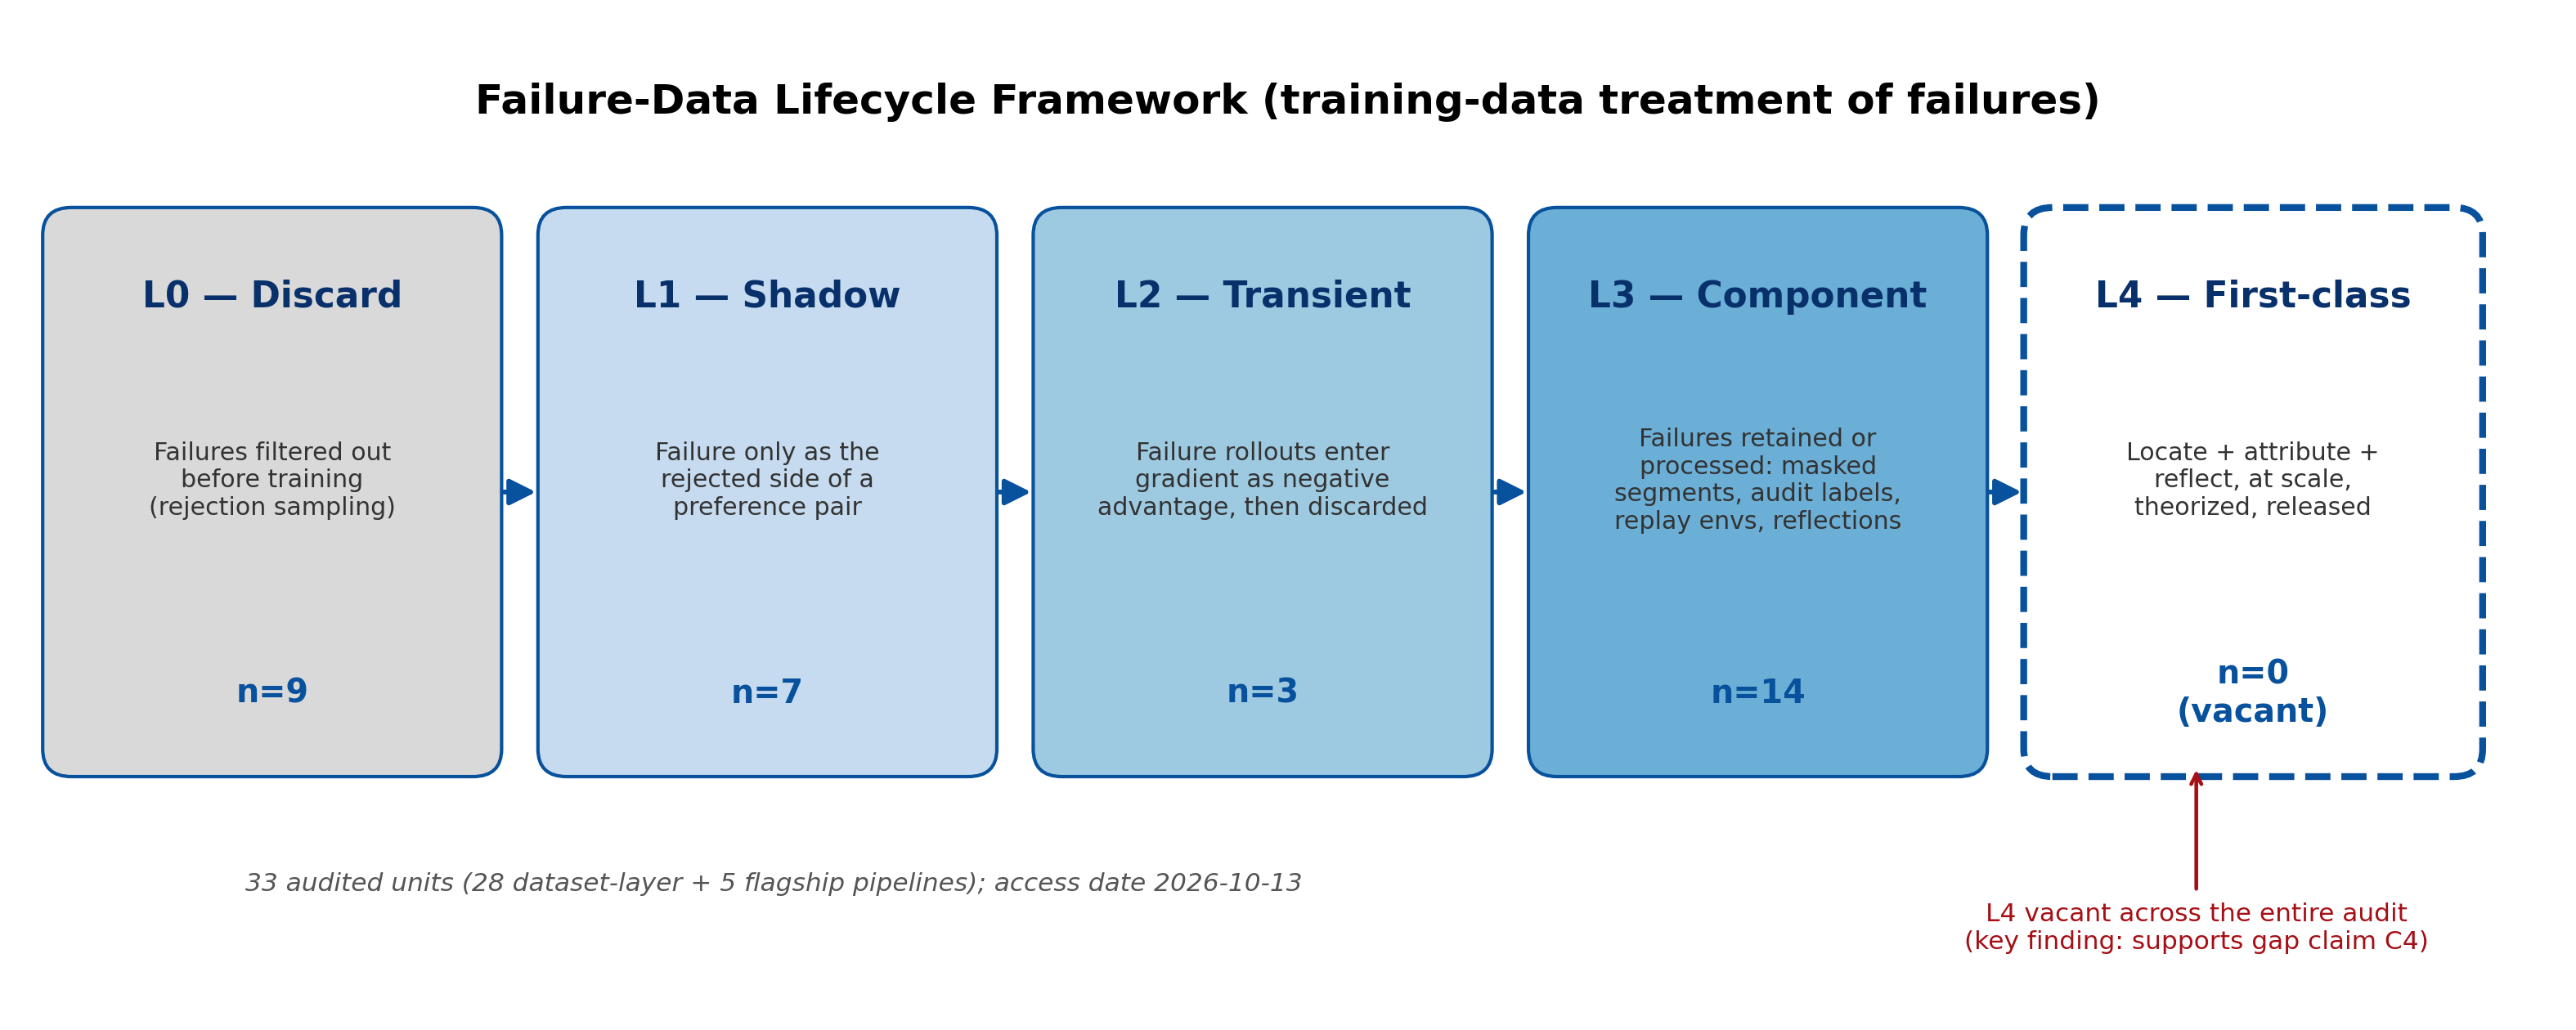
\includegraphics[width=0.95\textwidth]{fig1_lifecycle_framework.png}
\caption{失败数据生命周期框架（L0--L4）。单元计数来自对 33 个单元的审计（28 个数据集层 + 5 条旗舰管线）；L4 级在整个审计中全部空缺——这本身即是本文的关键发现。}
\label{fig:lifecycle}
\end{figure}

两条编码纪律贯穿始终。第一，L0--L4 是序数量表：我们报告频数与中位数，从不报告均值。第二，「未披露」绝不蕴含「不存在」：披露不对称被视为效度威胁而非证据（第~\ref{sec:limitations}~节）。

\section{审计方法}\label{sec:method}

\subsection{设计与语料}

本研究是对公开来源的文档审计；不涉及人类受试者。证据分两层汇集，于 2026-10-13 锁定（数据版本 audit-v1.0）。

\textbf{语料 A（数据集层，$n{=}28$）}覆盖五个阶段的开源训练配方与数据集，各锚定一手来源：预训练——Dolma \cite{ai22024dolma}、FineWeb \cite{hf2024fineweb}；SFT/蒸馏——DeepSeek-R1 \cite{deepseek2025r1}、Llama 2 \cite{touvron2023llama2}、Llama 3 \cite{grattafiori2024llama3}、OpenR1-Math-220k \cite{hf2025openr1}、Bespoke-Stratos \cite{bespokelabs2025stratos}、OpenMathReasoning \cite{nvidia2025omr}、OpenMathInstruct-2 \cite{nvidia2024omi2}；偏好对齐——Llama 3 DPO \cite{grattafiori2024llama3}、Qwen3 \cite{qwen2025qwen3}、Tulu 3 \cite{lambert2025tulu3}、HH-RLHF \cite{anthropic2022hhrlhf}、SmolLM2 \cite{hftb2024smoltalk}、GLM-4.5 MIPO \cite{zai2025glm45}；RL——R1 中实现的 GRPO \cite{deepseek2025r1}、DAPO \cite{yu2025dapo}；以及学术例外——PRM800K \cite{lightman2023verify}、Math-Shepherd \cite{wang2024mathshepherd}、LEMA \cite{an2023lema}、ETO \cite{song2024eto}、UltraInteract \cite{yuan2024ultrainteract}、UltraFeedback \cite{openbmb2023ultrafeedback}、ProcessBench \cite{zheng2024processbench}、PRMBench \cite{song2025prmbench}、OpenR1-Math-Raw \cite{openr12025mathraw}、NPO 的遗忘集 \cite{zhang2024npo}、SPAR 平台的 f26 人工标注智能体失败轨迹集 \cite{spar2026f26}。纳入要求：可核实的一手文档（论文、官方数据卡或官方仓库）、社区采用或方法论代表性、且披露不晚于 2026-10-13。仅由媒体报道支撑的单元被排除；一个广为流传的具身失败分析数据集经多次定向检索仍无法在一手来源中定位，被整体移出证据链——具身失败推理改经可核验的一手工作引用 \cite{duan2024aha}。

\textbf{语料 B（管线层，$n{=}5$）}覆盖蒋云岗 2026 年 7 月讲话之后发布的旗舰，各锚定第一方文档：GPT-6 Astra 的系统卡 \cite{openai2026gpt6}、Claude Opus 5.5 的系统材料 \cite{anthropic2026claude}、GLM-5 技术报告（GLM-5.3 披露的锚点）\cite{zai2026glm5}、MiMo-V2.6 \cite{xiaomi2026mimo}、DeepSeek-V4.1-Flash \cite{deepseek2026v41}。这是饱和目的抽样——五者即公认的闭源与开源旗舰第一梯队——而非概率抽样；结论相应限定于\emph{已披露实践}。一个文献语料（上述五个家族）与一次覆盖 2026 年 8--10 月的 arXiv 复查构成其余材料。

\subsection{流程}

编码遵循如下管线：检索 $\rightarrow$ 纳入/排除 $\rightarrow$ 一手来源核验 $\rightarrow$ 机制级编码 $\rightarrow$ 信度复查 $\rightarrow$ 数据锁定。44 条机制记录（语料 A 30 条、语料 B 14 条）中的每一条都携带逐字或摘录级引文及章节锚点、来源层级、置信度评级与冲突规则引用。五条冲突规则裁决判断：多级单元以最高级为主码（CR1）；一手来源压倒二手来源（CR2）；同一厂商的不同版本拆分为独立记录（CR3）；不可判定的判据给低置信度、绝不臆断（CR4）；未披露绝不编为 L0（CR5）。对语料 B，每个 L2 及以上的编码锚定一条不超过 50 词的逐字引文。

\subsection{验证修正}

由于上游证据链曾包含两处传播性错误，我们对所有实际承重的数字执行了验证闸门。PRS 引自经核验的一手来源（arXiv:2606.26027），分析器模型更正为 gpt-5-mini，收益表述为 $+22.25$ 分（25.75 对 3.50），绝不换算为倍数 \cite{hao2026prs}。DAPO 以其正确的标识符（arXiv:2503.14476）引用 \cite{yu2025dapo}。本文所有头条数字均可追溯至锁定分析，并经该闸门复核。

\subsection{信度与质量闸门}

全部 33 个单元由单一编码员依编码手册的全称量词判据编码。为缓解单编码员风险，编码手册、边界案例登记册（14 例登记在案）与完整机制级编码表随本文发布，使每一个判断都可被独立重新裁定；分层 20\% 样本（语料 A 六个单元、一条完整旗舰、一个文献家族）的分层 20\% 样本（语料 A 六个单元、一条完整旗舰、一个文献家族）的盲法评分者内重编码已预注册并排期，原始一致率与 Cohen's $\kappa$（目标 $\kappa \ge .70$）将随下一个数据版本报告。二手层证据（新闻报道，如 \cite{waic2026}）仅限于动机，从不支撑任何主张。

\subsection{效度威胁}

我们标记五项威胁——双向的披露偏差、单一编码员、序数量表、截断的时间窗、摘录级引文——并在第~\ref{sec:limitations}~节处理。

\section{结果}\label{sec:results}

横跨 33 个单元与 44 条机制记录，全语料分布为 L0 $\times$9（27.3\%）、L1 $\times$7（21.2\%）、L2 $\times$3（9.1\%）、L3 $\times$14（42.4\%）、L4 $\times$0，未披露单元为零，序数中位数为 L2。我们按研究问题报告结果：数据集层、管线层与空缺扫描；有效性论证基于文献，已在 2.1--2.3 节处理。

\subsection{数据集层：失败数据的系统性降格}

\begin{table}[t]
\centering
\caption{语料 A（数据集层）：失败数据生命周期级别 $\times$ 训练阶段（$n{=}28$ 个单元）。}
\label{tab:corpusA}
\small
\begin{tabular}{lcccccc}
\toprule
级别 & 预训练 & SFT & 偏好 & RL & 学术 & 合计 (\%) \\
\midrule
L0 丢弃   & 2 & 7 & 0 & 0 & 0 & \textbf{9 (32.1\%)} \\
L1 影子    & 0 & 0 & 6 & 0 & 1 & \textbf{7 (25.0\%)} \\
L2 瞬时 & 0 & 0 & 0 & 2 & 0 & \textbf{2 (7.1\%)} \\
L3 组件 & 0 & 0 & 0 & 0 & 10\textsuperscript{*} & \textbf{10 (35.7\%)} \\
L4 一等公民 & 0 & 0 & 0 & 0 & 0 & \textbf{0 (0.0\%)} \\
未披露 & 0 & 0 & 0 & 0 & 0 & \textbf{0} \\
\midrule
\textbf{合计} & 2 & 7 & 6 & 2 & 11 & \textbf{28} \\
\bottomrule
\end{tabular}

\vspace{2pt}
\par\noindent{\footnotesize \textsuperscript{*}含两个评测侧参照单元（ProcessBench、PRMBench）；剔除后 L3 $=$ 8/28。}
\end{table}

\begin{figure}[t]
\centering
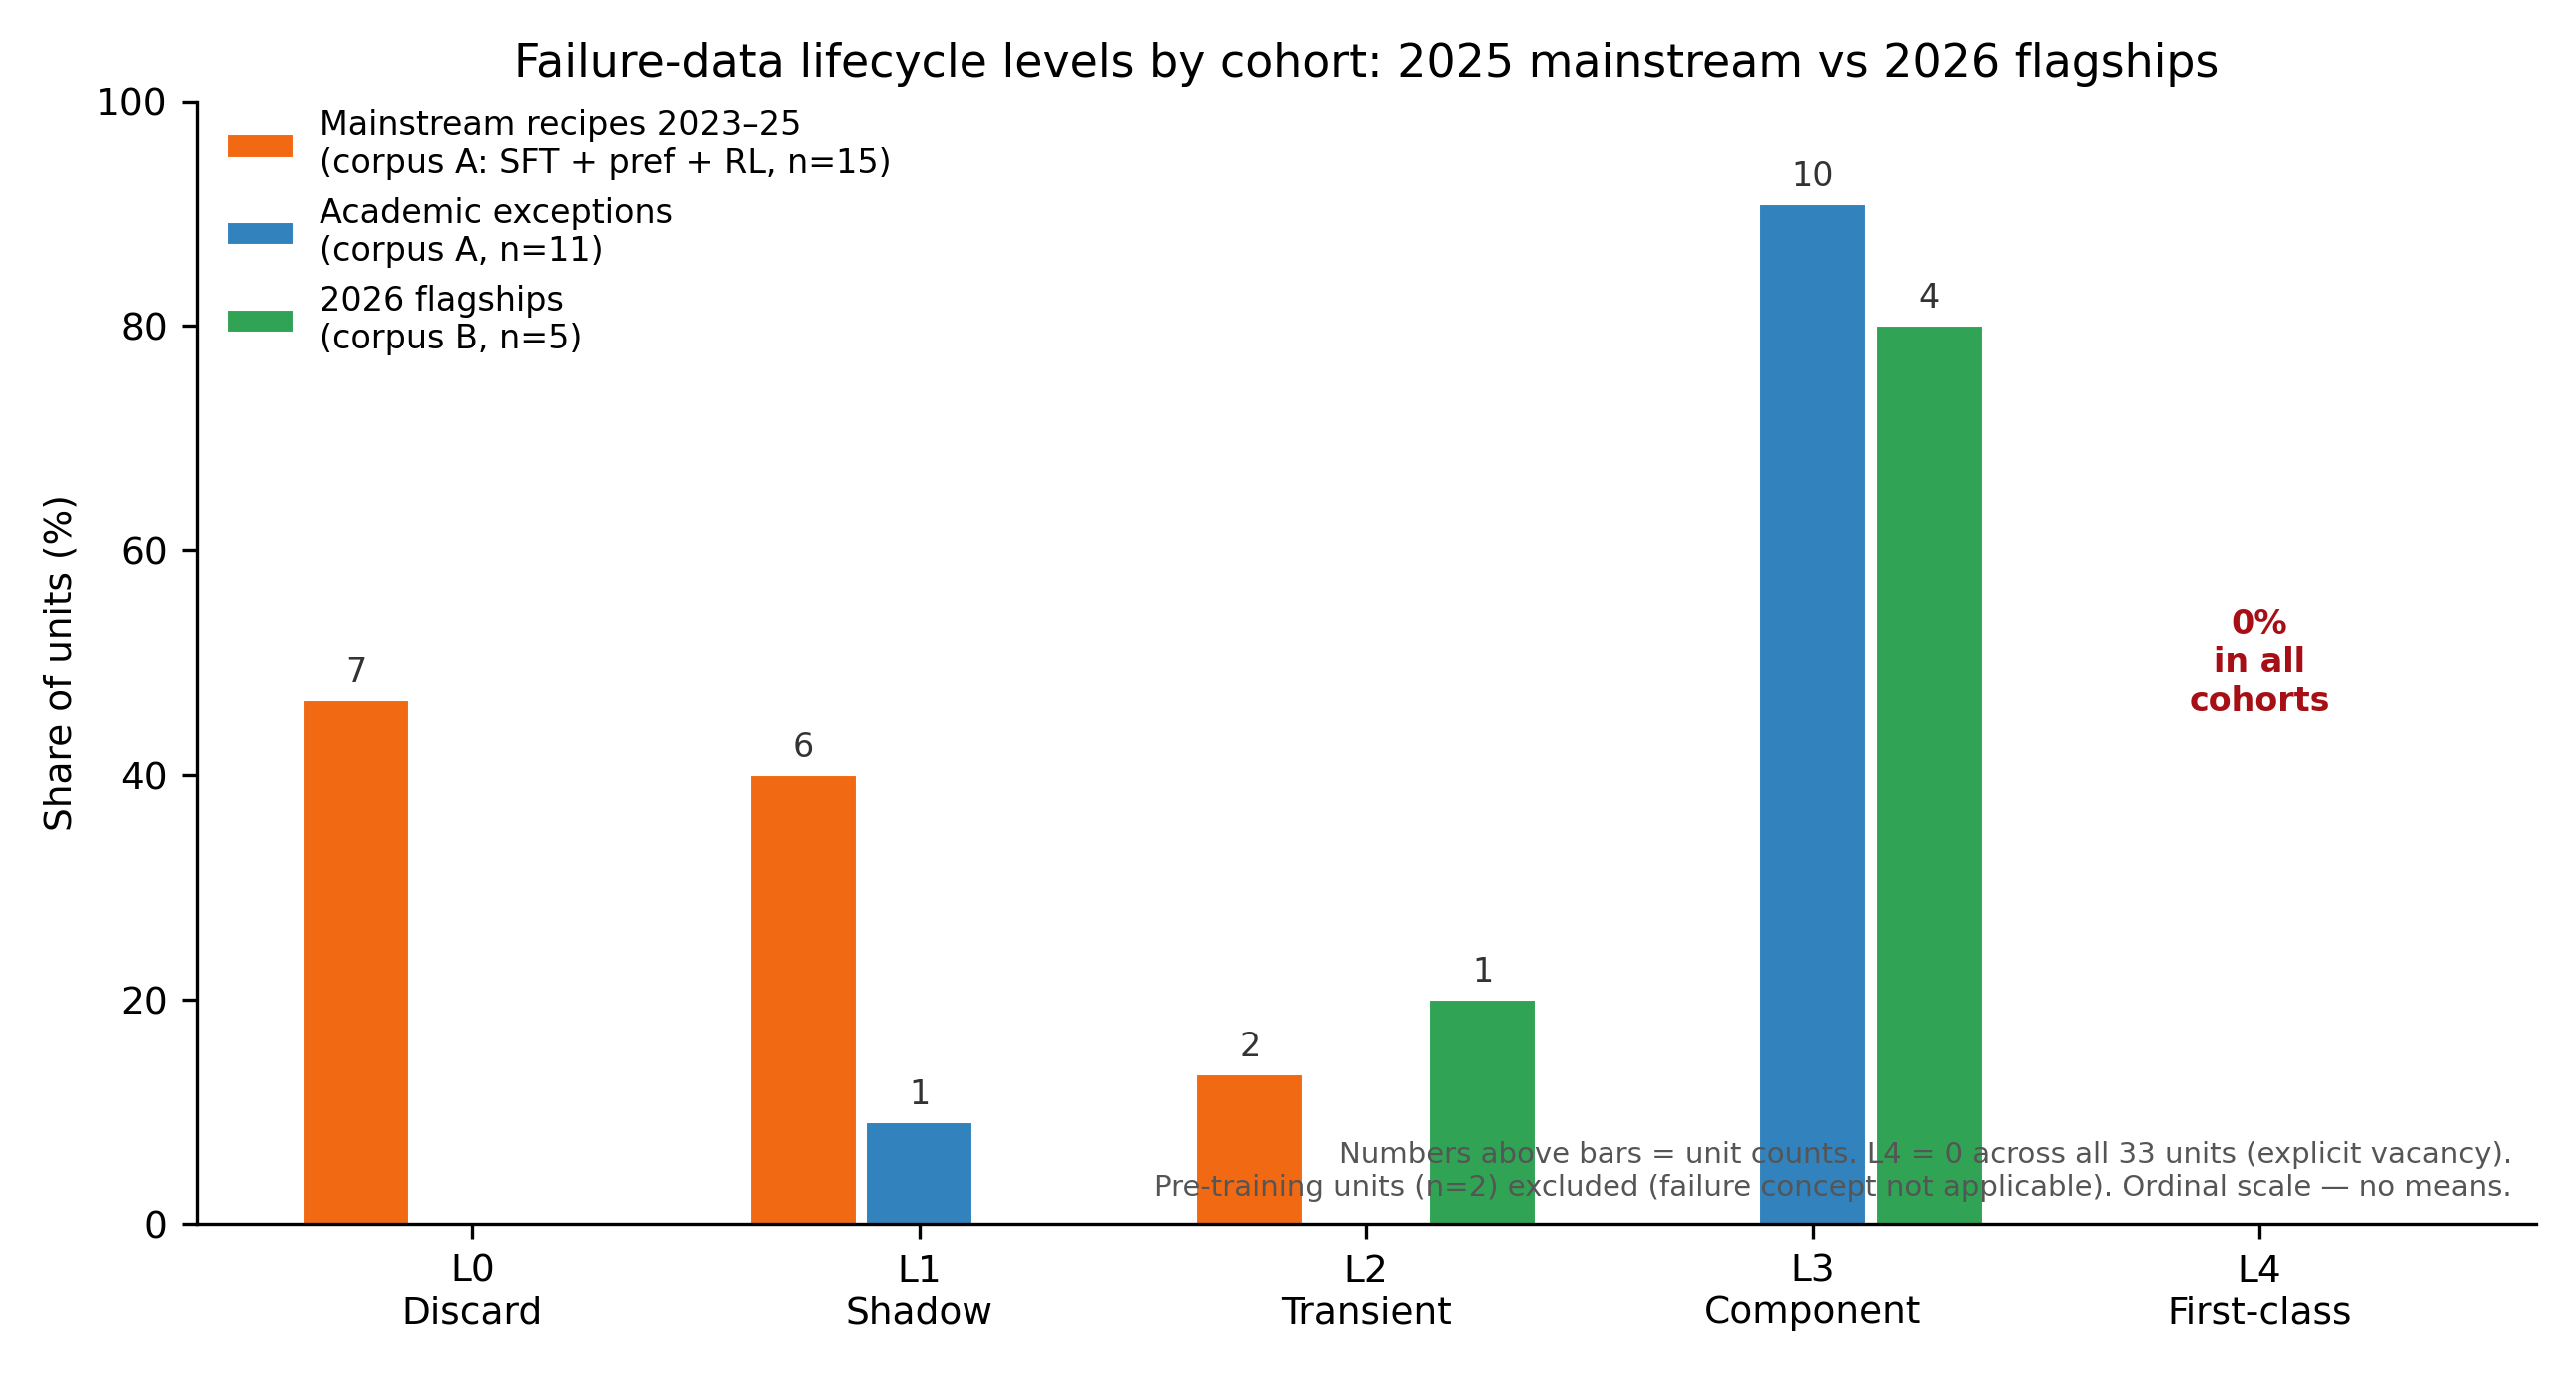
\includegraphics[width=0.95\textwidth]{fig2_level_distribution.png}
\caption{各队列失败数据生命周期级别的分布：2023--25 主流配方（$n{=}15$）、学术例外（$n{=}11$）、2026 旗舰（$n{=}5$）。柱上数字为单元计数；所有队列中 L4 $=$ 0。预训练单元不计入（失败概念不适用）。}
\label{fig:levels}
\end{figure}

表~\ref{tab:corpusA} 与图~\ref{fig:levels} 显示出按阶段的清晰分层。\textbf{全部七个 SFT/蒸馏单元都是 L0}：拒绝采样式的失败轨迹丢弃是 2023--25 SFT 数据生产的默认操作（R1、Llama 2/3、OpenR1-Math、Bespoke-Stratos、OpenMathReasoning、OpenMathInstruct-2）。偏好阶段一律 L1——六分之六，包括 MIPO：它对负样本强度定级，但不做定位、归因或反思，因而更恰当的描述是影子层级的上界，而非组件设计。RL 阶段到达 L2；DAPO 记录为多级 L0+L2，其全失败组移除构成丢弃被制度化的算法级证据。限定于主流子集（SFT + 偏好 + RL，$n{=}15$）：\textbf{0/15 个单元达到 L3，该子集的序数中位数为 L1}。每一个 L3 单元都位于学术例外层（10/11，其中 SPAR f26 为低置信编码）——社区显然知道如何构建富含失败样本的数据集，也同样显然不在主流配方中交付它们。两处边界判读值得注意：两个评测侧 L3 单元证明定位型与归因型的数据存在，但服务于评测而非训练——我们编码的是数据形式，而非用途等价（OpenMathInstruct-2 的边界判读见第~\ref{sec:codebook}~节）。

\subsection{管线层：一场未被命名的代际转变}

\begin{table}[t]
\centering
\caption{语料 B（五条 2026 旗舰）：生命周期级别 $\times$ 子维度（$n{=}5$）。}
\label{tab:corpusB}
\resizebox{\textwidth}{!}{%
\begin{tabular}{lccccccccc}
\toprule
模型（发布） & 主码 & 多级 & 粒度 & 归因 & 反思 & 领域 & 开放性 & 载体 & 置信度 \\
\midrule
GPT-6 Astra（09-03） & \textbf{L2} & L0+L2 & 轨迹 & 无 & 无 & 对齐 & 未发布 & 审计回路 & 高\textsuperscript{\dag} \\
Claude Opus 5.5（09-22） & \textbf{L3} & --- & 轨迹 & 二元 & 无 & 对齐 & 未发布 & 审计回路 & 中 \\
GLM-5.3（2026 H2） & \textbf{L3} & L0+L3 & \textbf{步骤} & 二元 & 无 & 能力 & 未发布 & 静态数据集 & 高 \\
MiMo-V2.6（09-22） & \textbf{L3} & --- & \textbf{步骤} & 二元 & \textbf{完整报告} & 对齐 & 未发布 & 静态数据集 & 高 \\
DeepSeek-V4.1-Flash（09-09） & \textbf{L3} & --- & 轨迹 & \textbf{根因} & 无 & 能力 & 未发布 & RL 环境 & 高 \\
\bottomrule
\end{tabular}}

\vspace{2pt}
\par\noindent{\footnotesize \textsuperscript{\dag}单元置信度取自主码机制（RL 惩罚，逐字引自系统卡）；监控/评测路由机制为中（摘录级引文）。}
\end{table}

表~\ref{tab:corpusB} 逐一标定各条旗舰的位置。\textbf{五分之四的单元是 L3；队列中位数为 L3。} GPT-6 Astra 是唯一低于 L3 的旗舰：其对失败的唯一训练侧使用是一个瞬时 RL 惩罚——``penalize cheating and unauthorized actions'' \cite{openai2026gpt6}——而失败信号被显式路由到监控与评测（路由去向有明示、属显式丢弃，故该机制编为 L0）。GLM-5.3 对错误做掩码而非删除：``Erroneous segments within trajectories are retained but masked out in the loss function, allowing the model to learn error correction behaviors'' \cite{zai2026glm5}，同时以错题本式的 RL 任务选择持续失败的上一代任务，并以二元归因区分模型错误与环境崩溃。MiMo-V2.6 是唯一三要素齐备的单元，从真实奖励作弊失败中合成训练样本，其形式 ``keeps the original error recognizable and makes the correction explicit'' \cite{xiaomi2026mimo}。DeepSeek-V4.1-Flash 在结构上最接近 L4：``we collect negative feedback and model failure cases submitted by internal employees at scale''，馈入 ``systematic replay of failures and targeted RL against observed model weaknesses'' \cite{deepseek2026v41}——有组织的采集、根因归因与能力域范围。Claude Opus 5.5 从 7,200 余个采集的智能体失败场景驱动训练改进，但仅限对齐领域 \cite{anthropic2026claude}（摘录级证据；此处为转述）。

\begin{table}[t]
\centering
\caption{子维度分布（单元级），语料 A 对语料 B。}
\label{tab:subdims}
\small
\begin{tabular}{llcc}
\toprule
子维度 & 取值 & 语料 A ($n{=}28$) & 语料 B ($n{=}5$) \\
\midrule
粒度 & 无 / 轨迹 / 步骤 / 因果 / 未定 & 3 / 18 / 6 / \textbf{0} / 1 & 0 / 3 / 2 / \textbf{0} / 0 \\
归因 & 无 / 二元 / 根因 / 未定 & 26 / \textbf{0} / 1 / 1 & 1 / 3 / 1 / 0 \\
反思 & 无 / 修正对 / 完整报告 / 未定 & 23 / 4 / \textbf{0} / 1 & 4 / 0 / \textbf{1} / 0 \\
领域 & 能力 / 对齐 / 兼有 / 未定 & 23 / 1 / 2 / 2 & 2 / 3 / 0 / 0 \\
开放性 & 已发布 / 未发布 & \textbf{11 / 17} & \textbf{0 / 5} \\
载体 & 无 / 偏好对 / 静态 / RL 环境 / 审计回路 & 9 / 8 / 9 / 2 / 0 & 0 / \textbf{0} / 2 / 1 / 2 \\
\bottomrule
\end{tabular}
\end{table}

表~\ref{tab:subdims} 展示\emph{载体迁移}，我们的第二个结构性发现。在 2023--25 主流队列中，6/15 个单元以偏好对承载失败；横跨五条旗舰的 14 条机制记录，\textbf{偏好对承载为 0}（审计回路 $\times$4、静态数据集 $\times$5、RL 环境 $\times$5）。同厂商记录对版本动态是决定性的：MIPO 的分级负样本（L1）在 GLM-5.x 中退役，其后训练链不含偏好优化阶段 \cite{zai2025glm45,zai2026glm5}；DeepSeek 自身的轨迹从 R1 的拒绝采样（2025-01，L0）走到 V4.1-Flash 的失败重放（2026-09，L3），拒绝采样阶段已消失 \cite{deepseek2025r1,deepseek2026v41}。

\begin{table}[t]
\centering
\caption{代际对比：2023--25 主流配方对 2026 旗舰。}
\label{tab:generations}
\small
\begin{tabular}{lccccccccc}
\toprule
队列 & $n$ & L0 & L1 & L2 & L3 & L4 & $\ge$L3 & 中位数 \\
\midrule
2023--25 主流（SFT+偏好+RL） & 15 & 7 (46.7\%) & 6 (40.0\%) & 2 (13.3\%) & 0 & 0 & \textbf{0 (0.0\%)} & L1 \\
2026 旗舰 & 5 & 0 & 0 & 1 (20\%) & 4 (80\%) & 0 & \textbf{4 (80.0\%)} & L3 \\
\bottomrule
\end{tabular}
\end{table}

表~\ref{tab:generations} 将这一转变形式化；探索性 Fisher 精确检验给出 $p = .001$（双侧；单侧相同）。我们强调告诫：饱和目的抽样、$n = 5$、序数数据、无随机化——承载论证的是分布与锚定引文，而非该检验。敏感性检验进一步收紧了主张：剔除低置信与边界单元后，主流队列 $\ge$L3 为 0/14、旗舰为 3/4（单侧 $p = .005$）；将预训练单元并入 2025 队列不改变结论（$p < .001$）；但将语料 A \emph{全部} 28 个单元与旗舰对比，$\ge$L3 为 10/28、$p = .089$（单侧）——代际对比的强度取决于「主流配方」的框定，因为学术例外层按构造就是一个反例层。因此我们主张的是\emph{主流已披露实践}中的代际转变，而非总体估计。

\subsection{空缺：三要素与开放性}

\begin{table}[t]
\centering
\caption{生命周期级别 $\times$ 三要素（全部 33 个单元）。}
\label{tab:elements}
\small
\begin{tabular}{lcccc}
\toprule
级别 & $n$ & 定位（步骤/因果） & 归因（二元/根因） & 反思（修正对/完整报告） \\
\midrule
L0 & 9 & 0 & 0 & 0 \\
L1 & 7 & 0 & 0 & 0 \\
L2 & 3 & 0 & 0 & 0 \\
L3 & 14 & 8 (57.1\%) & 5 (35.7\%) & 5 (35.7\%) \\
L4 & 0 & --- & --- & --- \\
\bottomrule
\end{tabular}
\end{table}

表~\ref{tab:elements} 显示三要素随级别共变——严格集中于 L3（如定位 8/14 对其余的 0/19；探索性 Fisher $p = .00022$；归因与反思 5/14 对 0/19，$p = .008$）——但联合满足三要素的\textbf{恰好一个单元，33 中之一（MiMo-V2.6）}，即便在 L3 内部也是十四分之一。各要素个体上仍然稀缺：因果粒度的定位在全语料缺席（0/33）；根因归因存在于语料 A 的一个评测侧单元（PRMBench）与一条旗舰（DeepSeek）；完整反思报告存在于一个单元（MiMo）。开放性沿一条制度断层线切分语料：失败数据已发布的 11 个单元\emph{全部}在学术侧（10 个学术例外，加上 HH-RLHF 已发布的被拒绝侧），而旗舰零发布（0/5）——MiMo 公开五条奖励作弊失败轨迹属于示例级披露，其约 7,000 个 RL 环境的开源不是失败数据的发布。

对两个语料的 L4 扫描返回 \textbf{0/33}，四条判据以结构化的方式失守：判据 (i) 三要素，仅 MiMo 满足；判据 (ii) 规模，MiMo 未披露；判据 (iii) 作为方法论的显式理论化，无任何厂商满足——DeepSeek 把整套装置表述为工程：``the marginal return of engineering the data and environment pipeline substantially exceeds that of algorithmic novelty'' \cite{deepseek2026v41}；判据 (iv) 公开发布，无旗舰满足。与 L4 失之交臂但最接近的，是 LEMA（要素大体齐备且已发布，但规模在 $10^4$、且处于主流配方之外）与 DeepSeek-V4.1-Flash（有组织的规模与根因归因，但未命名、未发布）。最后是程序性佐证：2026 年 8--10 月的 arXiv 复查未发现大规模失败数据集或工业级失败反思方法论的论文；相邻的命中关乎失败检测 \cite{zhang2026foresight}。

\section{讨论}\label{sec:discussion}

\subsection{作为发现的空缺}

写编码手册时 L4 级就被预期为空，而审计系统地确认了这一点。因此局面既非「失败数据没有用」——各方法论家族提供了受控的正面证据（第~\ref{sec:background}~节）——也非「没人想要」：一位资深政策人物在 2026 年 7 月公开点名 \cite{waic2026}，五条旗舰管线中的四条现已包含失败组件。在所审计的披露层与 2026-10-13 证据窗口之内，一等公民级失败数据是一块\emph{无人占据的高地}：它在小规模上被证明，在公共话语中已被命名，最弱的模型维度恰恰需要它，却仍无人将其认领为方法论。空缺是可证伪且带时间戳的：十二个月内出现满足全部四条 L4 判据的公开发布即可将其驳倒，而我们恰将其列为监测指标。

\subsection{最佳载体也许是环境，而非数据集}

载体迁移（表~\ref{tab:subdims}）提示这个领域已用基础设施投票。偏好对载体——影子形式——未能走出它的时代：MIPO，其最系统的设计，被退役而非被放大 \cite{zai2025glm45}。三条旗舰载体各承载一个要素：MiMo 的反思-修正数据承载反思，DeepSeek 的重放环境承载归因驱动的定向，GLM 的掩码片段承载定位。失败数据的终局形态也许不是静态标注语料，而是一个\emph{闭环}——采集、归因、重放、再训练——正如 DeepSeek 的披露所暗示 \cite{deepseek2026v41}。我们持双重立场。对工业管线，环境加重放确实可能占优：它们使失败数据保持在策略分布上（on-policy）并保持时新。但闭环就其构造而言是私有的；若社区终要以累积的方式研究失败数据方法论，静态、开放许可、三元标注的语料仍是唯一可共享的形式——而 PRS 证明，反思性\emph{文本}数据用普通的 SFT 损失即可训练、已经有效 \cite{hao2026prs}。两种形式、以及它们之间的桥，都应进入路线图。

\subsection{对最弱维度的启示}

我们的审计度量的是实践而非效果，我们抵制超出证据的因果推断。激励的契合仍然醒目：泛化与校准正是当前训练最弱的维度，也恰是失败数据可发挥候选信号作用的维度，依据是第 1 节的后验收缩论证，依据是第~\ref{sec:intro-arg}~节的后验收缩论证。RLVR 似乎锐化 pass@1 而不扩展 pass@$k$ \cite{yue2025rlvr}；幻觉表现得像被自信猜测奖励强化的校准失败 \cite{kalai2025halluc}；后训练可测量地损害置信度校准 \cite{he2023calibration,xie2026know}。在归因失败上训练，形式上就是在\emph{能力边界}上训练——一个校准良好的模型必须拒绝作答的区域。现有最强的提示是 PRS 的双重未见结果（12.00 对 0.00）\cite{hao2026prs}；确立失败数据在规模上的泛化--校准收益是一个开放的实验纲领，我们路线图中的评测组件即为启动该纲领而设计。

\subsection{验证器依赖}\label{sec:verifier}

失败数据的定义继承自验证器，而验证器可以被博弈。奖励作弊是一种\emph{假成功}——不经因果归因，无论当正样本还是负样本来训练都有毒。旗舰的组件大多恰是对这一问题的回答：MiMo 的在线评分器联合检查成功与失败的 rollout，将确认作弊的通过清零、转化为失败 \cite{xiaomi2026mimo}；GLM 封堵求解轨迹中的奖励捷径，并区分模型错误与环境崩溃 \cite{zai2026glm5}；DeepSeek 将作弊与环境崩溃记录为失败轨迹、回馈给 RL 框架 \cite{deepseek2026v41}。开放问题是无验证器领域：在成功无法自动核查的领域，失败归因需要新的工具；没有它们，该方法论就走不出数学与代码这类可验证领域。

\subsection{局限}\label{sec:limitations}

五项局限约束我们的主张。(1) \emph{双向披露偏差}：未披露的失败实践会使我们的 L 级别被低估；厂商的粉饰会使组件被高估。因此全部结论限定于已披露实践，且我们发布锚定引文供读者重新裁定。(2) \emph{单一编码员}：本审计是一位编码员对公开编码手册的应用；评分者内 $\kappa$ 尚待完成（第~\ref{sec:method}~节），且不存在评分者间信度。(3) \emph{序数纪律}：L0--L4 只支持中位数与分布；我们不报告均值或区间统计。(4) \emph{时间截断}：语料是移动靶标的一个 2026 年秋季快照；单元按版本锚定，代际对比按队列框定（全语料敏感性 $p = .089$ 标出统计主张的边界）。(5) \emph{引文置信度}：逐字引文锚定全部高置信的语料 B 编码；三条语料 B 机制与多数语料 A 锚点依赖摘录级证据，对它们我们转述而不引用。

\section{路线图：让失败数据成为一等公民}\label{sec:roadmap}

审计的厂商映射（表~\ref{tab:roadmap}）显示哪些组件已存在、哪些缺失；五家厂商无一集齐全部组件，且开放语料组件在整个行业空缺。

\begin{table}[t]
\centering
\caption{路线图组件 $\times$ 旗舰覆盖（来自审计的子维度记录）。}
\label{tab:roadmap}
\footnotesize
\setlength{\tabcolsep}{3.5pt}
\begin{tabular}{p{2.9cm}p{2.4cm}p{2.6cm}p{2.4cm}p{1.9cm}p{1.7cm}}
\toprule
组件 & MiMo & DeepSeek & GLM-5.3 & Claude & GPT-6 \\
\midrule
(a) 三元采集/标注协议 & 部分（反思-修正样本，仅作弊域） & 部分（员工提交 + 分类，无反思文本） & 部分（掩码保留，无反思） & 无 & 无 \\
(b) 去毒化清洗与因果归因 & 有（作弊通过清零；剔除基础设施故障） & 有（作弊/崩溃记为失败） & 部分（二元模型-环境剔除） & 部分（缺陷环境归因） & 未披露 \\
(c) 验证器依赖处理 & 有（成功/失败联合评分） & 部分（检查代理标记） & 有（奖励捷径封堵） & 未披露 & 未披露 \\
(d) 开放语料与共享协议 & 无（开放环境 $\neq$ 开放失败数据） & 无 & 无 & 无 & 无 \\
\bottomrule
\end{tabular}
\end{table}

由此映射，我们具体给出缺失的基础设施：

\begin{enumerate}
\item \textbf{三元数据模式。} 失败记录作为一等对象，含三个必填字段——错误类型（定位到步骤或因果粒度）、根因、更正文本——连同溯源信息（任务、策略版本、验证器判定）。该模式不依赖特定载体：适用于静态数据集、偏好对扩展与环境日志。
\item \textbf{采集与标注协议。} 谁采集失败（用户、员工、rollout），如何按多样性而非数量抽样，由哪个分析器标注——并披露分析器模型，一个我们的验证链表明至关重要的细节 \cite{hao2026prs}。
\item \textbf{去毒化清洗与因果归因。} 一个强制性的训练前阶段，把假成功（奖励作弊）、基础设施故障与有价值的模型失败区分开，遵循旗舰先例（第~\ref{sec:verifier}~节）。
\item \textbf{验证器依赖处理。} 对「通过但可疑」轨迹的双重评分协议，以及面向无验证器领域失败归因的研究纲领。
\item \textbf{开放语料与共享协议。} 生态中唯一保留失败的大规模发布是 OpenR1-Math-Raw（$\sim$10\textsuperscript{6} 条原始轨迹，L3 且开放性=已发布但要素不全）\cite{openr12025mathraw}；我们倡议社区在这样的原始种子之上构建三元标注层，配以许可与溯源约定——当前没有厂商从事此项活动（表~\ref{tab:roadmap}d）。
\item \textbf{一项评测基准。} 对使用与不使用匹配失败数据训练的模型进行受控比较，在分布外泛化（双重未见设计，遵循 \cite{hao2026prs}）与校准（置信度--正确性对齐）上评分，外加度量定位与归因能力的「失败素养」任务（扩展 \cite{zheng2024processbench,song2025prmbench}）。
\end{enumerate}

由审计得出可证伪的预测：十二个月内无 L4 发布将延长空缺；偏好对份额持续近零将确认载体迁移；第一家将其失败管线理论化为方法论的厂商将占据空缺的层级。

\section{结论}\label{sec:conclusion}

我们审计了 LLM 训练实践如何对待失败数据，并发现一个结构化的悖论。方法论在小规模上被证明、话语已为之命名，然而在 33 个受审单元中，最高生命周期层级为空（0/33），2023--25 主流从未升到瞬时失败梯度之上（$\ge$L3 为 0/15；全部 SFT 单元为纯丢弃），而 2026 旗舰——确实运行失败组件（4/5 在 L3）——将其保持局部、未命名、未发布，且已抛弃曾隐式承载失败的偏好对载体（0/14 个旗舰机制）。成功给方向；失败给精度；而当前实践，就其已披露的一切而言，把精度扔掉了。审计工具——生命周期编码手册、边界案例登记册与开放编码记录——随本文发布，使这一空缺可以被公开监测，也可以被公开驳倒。

\section*{数据与材料可得性}

编码手册（五级生命周期判据加六个子维度）、14 例边界登记册、机制级编码表（44 条记录，含锚定引文、章节锚点、来源层级与置信度评级）、复现脚本（\texttt{coding\_data.py}）与两图随本文打包，作为补充材料发布。 % TODO(作者)：投稿前替换为永久仓库 URL/DOI（建议 GitHub + Zenodo）

\section*{代码可得性}

复现脚本与编码数据集（CSV）随补充材料以开放许可发布。 % TODO(作者)：确认许可（如代码 MIT、数据 CC-BY 4.0）与仓库 URL。

\section*{资助}

本研究未接受外部资助。 % TODO(作者)：确认。

\section*{利益冲突}

作者隶属余玉桂战略研究室（独立研究机构）；与受审计的各厂商不存在可能影响本工作的财务或个人关系。 % TODO(作者)：确认措辞。

\section*{AI 辅助披露}

本研究的研究与写作过程借助了大语言模型系统作为研究与写作协作者（文献检索、编码表整理与起草）。全部证据单元、编码判断、引文与数字均由人类作者挑选、核验并对其负责，遵循 4.3 节所述的验证闸门；审计上游的两处传播性错误正是被该闸门捕获并更正的。本披露为自愿作出；arXiv 政策要求作者对所有内容负责，并惩戒未经核查的 AI 生成材料。

\bibliographystyle{unsrtnat}
\bibliography{references}

\end{document}
